\documentclass[12pt,letterpaper]{article}

%%%%%%%%%%%%%%%%% common packages are included here %%%%%%%%%%%%%%%%%
\usepackage{graphicx}
\usepackage{epstopdf}
\usepackage{tabularx}
\usepackage[lofdepth,lotdepth]{subfig} % subfloat
\usepackage{bm} % bold math
\usepackage{color}
\usepackage[centertags]{amsmath}
\usepackage{mathrsfs}
\usepackage{amsmath}
\usepackage{mathtools}
\usepackage{amssymb}
\usepackage{amsfonts}
\usepackage{amssymb}
\usepackage{amsthm}
\usepackage{newlfont}
\usepackage{textcomp,gensymb} % for \textcelsius, \textdegree, and \degree
\usepackage{syntonly}

%%%%%%%%%%%%%%%%%%%% some declaration %%%%%%%%%%%%%%%%%%%%%
\DeclareGraphicsExtensions{.pdf,.png,.jpg,.eps}
\graphicspath{{./figures/}}

%%%%%%%%%%%%%%%%%%% new commands are defined here %%%%%%%%%%%%%%%%%%%%%
\newcommand{\dg}{$^{\circ}$} % degree symbol
\newcommand{\iang}{\AA$^{-1}$} % inverse Angstrom symbol
\newcommand{\degC}{$^{\circ}\mathrm{C}$} % degree Celcius
\newcommand{\Eq}[1]{Eq.\,(\ref{#1})} % reference to an equation

% Some mathematical (physical) quantities and symbols that are used often
\newcommand{\xhat}{\mathbf{\hat{x}}}
\newcommand{\yhat}{\mathbf{\hat{y}}}
\newcommand{\zhat}{\mathbf{\hat{z}}}
\newcommand{\kin}{\mathbf{k}_{\mathrm{in}}}
\newcommand{\kout}{\mathbf{k}_{\mathrm{out}}}
\newcommand{\Tat}{\mathrm{Tat}}
\newcommand{\DOPC}{\mathrm{DOPC}}
\newcommand{\cm}{\mathrm{cm}}

% To simplify some formatting issues
\newcommand{\pars}[1]{\mathopen{}\left( #1 \right)\mathclose{}} % () without extra spaces due to \left and \right
\newcommand{\angles}[1]{\left\lange #1 \right\rangle}%      <>
\newcommand{\braces}[1]{\left\lbrace #1 \right\rbrace}%     {}
\newcommand{\bracks}[1]{\left\lbrack #1 \right\rbrack}%     []
\newcommand{\ds}[1]{\displaystyle{#1}}%
\newcommand{\+}{^{\dagger}}%                                
\newcommand{\partiald}[3][]{{\partial^{#1}#2 \over \partial {#3}^{#1}}}%


\newcommand{\z}[1]{z_\textrm{#1}}
\newcommand{\zPC}{z_\textrm{PC}}
\newcommand{\zCG}{z_\textrm{CG}}
\newcommand{\zHC}{z_\textrm{HC}}
\newcommand{\zCHthree}{z_{\textrm{CH}_3}}
\newcommand{\zTat}{z_\textrm{Tat}}
\newcommand{\zphos}{z_\textrm{phos}}

\newcommand{\sigmaPC}{\sigma_\textrm{PC}}
\newcommand{\sigmaCG}{\sigma_\textrm{CG}}
\newcommand{\sigmaHC}{\sigma_\textrm{HC}}
\newcommand{\sigmaCHthree}{\sigma_{\textrm{CH}_3}}
\newcommand{\sigmaTat}{\sigma_\textrm{Tat}}

\newcommand{\cPC}{c_\textrm{PC}}
\newcommand{\cCG}{c_\textrm{CG}}
\newcommand{\cCHthree}{c_{\textrm{CH}_3}}
\newcommand{\cTat}{c_\textrm{Tat}}

\newcommand{\PPC}{P_\textrm{PC}}
\newcommand{\PCG}{P_\textrm{CG}}
\newcommand{\PCHthree}{P_{\textrm{CH}_3}}
\newcommand{\PCHtwoCH}{P_{\textrm{CH}_2+\textrm{CH}}}
\newcommand{\PHC}{P_\textrm{HC}}
\newcommand{\PTat}{P_\textrm{Tat}}
\newcommand{\PW}{P_\textrm{W}}

\newcommand{\VHC}{V_\textrm{HC}}
\newcommand{\VHL}{V_\textrm{HL}}
\newcommand{\VL}{V_\textrm{L}}
\newcommand{\VTat}{V_\textrm{Tat}}
\newcommand{\VPC}{V_\textrm{PC}}
\newcommand{\VCG}{V_\textrm{CG}}
\newcommand{\VCHtwoCH}{V_{\textrm{CH}_2+\textrm{CH}}}
\newcommand{\VCHthree}{V_{\textrm{CH}_3}}
\newcommand{\VCHtwo}{V_{\textrm{CH}_2}}
\newcommand{\VCH}{V_\textrm{CH}}

\newcommand{\RPC}{R_\textrm{PC}}
\newcommand{\RCG}{R_\textrm{CG}}
\newcommand{\RTat}{R_\textrm{Tat}}

\newcommand{\RTL}{R_\textrm{T/L}}

\newcommand{\AL}{A_\textrm{L}}

\newcommand{\hTat}{h_\mathrm{Tat}}

\newcommand{\DC}{D_\textrm{C}}
\newcommand{\DB}{D_\textrm{B}}
\newcommand{\DPP}{D_\textrm{PP}}
\newcommand{\DHH}{D_\textrm{HH}}









\newcommand{\CH}[1]{\textrm{CH}_#1}

\newcommand{\rhoW}{\rho_\textrm{W}}

\newcommand{\dx}{\mathop{dx}}
\newcommand{\dz}{\mathop{dz}}
\newcommand{\dr}{\mathop{dr}}


\usepackage[pdftex]{hyperref}
%\setlength{\oddsidemargin}{0cm} \setlength{\topmargin}{0cm}
%\setlength{\textheight}{22cm} \setlength{\textwidth}{16cm}
%-----------------------------------------------------------------

\begin{document}
\today

%%%%%%%%%%%%%%%%%%%%%%%%%%%%%%%%%%%%%%%%%%%%%%%%%%%%%%%%%%%%%%%%%%%%%%%%%%%%%%%
\section{Analysis of Diffuse Scattering}
\subsection{Theory}
This section briefly describes NFIT analysis. 

%%%%%%%%%%%%%%%%%%%%%%%%%%%%%%%%%%%%%%%%%%%%%%%%%%%%%%%%%%%%%%%%%%%%%%%%%%%%%%%
\subsection{Results}
Show X-ray data. Show fitting boxes.
Show the Kc values.
Also, show the resultant
form factors, which qualitatively show the membrane thinning.

%%%%%%%%%%%%%%%%%%%%%%%%%%%%%%%%%%%%%%%%%%%%%%%%%%%%%%%%%%%%%%%%%%%%%%%%%%%%%%%
\newpage
\section{Modeling the Bilayer Structure}
In the case of X-rays, the features with the most contrast are the 
electron-dense headgroups, providing the head-head spacing $\DHH$,
as well as the terminal methyl groups in the bilayer center.
Modeling of the bilayer structure was done similarly to the SDP model 
\cite{ref:Kucerka08}. 

Parsing of DOPC into lipid components is shown in
Fig~\ref{fig:dopc_schematic}. The phosphate/choline (PC) and 
carbonyl/glycerol (CG) groups together make up the lipid headgroup
whereas the hydrocarbon chain region
is divided into two components, the methylene and methine groups 
combination ($\CH{2}$+CH) and terminal methyl group ($\CH{3}$). 
We combine methylene ($\CH{2}$) and methine groups (CH) in order to avoid 
proliferation of 
fitting parameters.
%------------------------------------------------------------------------------
\begin{figure}[htbp]
  \centering
  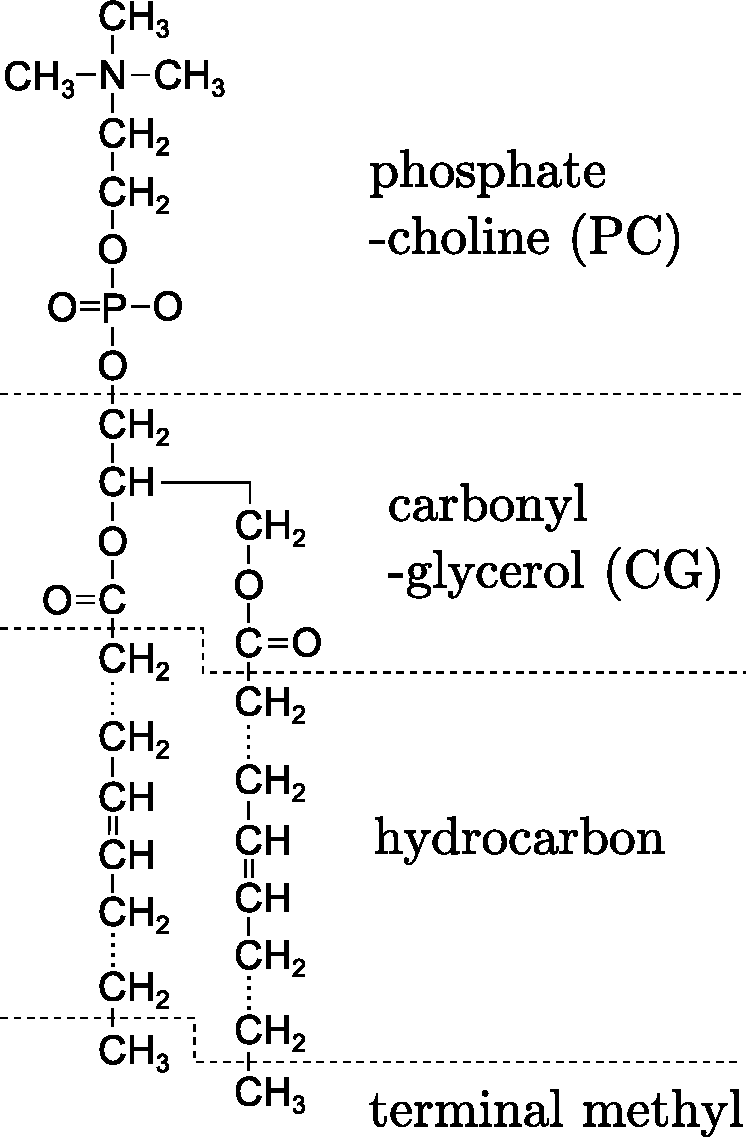
\includegraphics[scale=0.7]{./figures/dopc_schematic.pdf}
  \caption{Schematic of DOPC showing each lipid component. The dash lines 
           show where the lipid is divided into different components. 
           The lipid headgroup
           is divided into two components, phophate-choline and carbonyl-glycerol. 
           The hydrocarbon chain region is also divided
           into two components, methelence+methine and terminal methyl groups.}
  \label{fig:dopc_schematic}
\end{figure}
%------------------------------------------------------------------------------


%%%%%%%%%%%%%%%%%%%%%%%%%%%%%%%%%%%%%%%%%%%%%%%%%%%%%%%%%%%%%%%%%%%%%%%%%%%%%%%
\subsection{Functional forms}
Our model for electron density profile (EDP)
of Tat/lipid bilayer system consists of six structrual subgroups 
(Fig.~\ref{fig:DOPC_EDP1}).
The volume probability distributions of components PC, CG, terminal
methyl groups ($\CH{3}$), and Tat are described by Gaussian functions,
\begin{equation}
  P_i(z)=\frac{c_i}{\sqrt{2\pi}}\pars{
    \exp\braces{-\frac{(z+z_i)^2}{2\sigma_i^2}}
	+ \exp\braces{-\frac{z-z_i)^2}{2\sigma_i^2}}
  },
\end{equation}
where $c_i$ is an integrated area underneath the curve and the two parts of the 
expression describe the two bilayer leaflets. The calculation of $c_i$ is 
explained below.

The hydrocarbon chain region (HC) is represented by error functions,
\begin{equation}
  \PHC(z) = \frac{1}{2}\bracks{
    \mathrm{erf}(z,-\z{HC},\sigmaHC) - \mathrm{erf}(z,\z{HC},\sigmaHC)
  },
\end{equation}
where
\begin{equation}
  \mathrm{erf}(z,z_i,\sigma_i)=\frac{2}{\sqrt{\pi}}
    \int_0^{\frac{z-z_i}{\sqrt{2\sigma}}} \dx e^{-x^2}.
\end{equation}
The volume probability distribution for the methylene and methine groups 
combination can then be expressed as
\begin{equation}
  \PCHtwoCH(z) = \PHC(z)-\PCHthree(z).
  \label{eq:modelA}
\end{equation}
This definition enforces the total probability $\PHC$ in the hydrocarbon
chain region to equal one, which in turn means that placement of Tat in the  
chain region is prohibited. We call the model defined by Eq.~(\ref{eq:modelA})
model A (better name?). To allow Tat to be placed inside the hydrocarbon
chain region, we also consider an alternative definition,
\begin{equation}
  \PCHtwoCH(z) = \PHC(z)-\PCHthree(z) - \PTat(z),
\end{equation}
where the volume probability of CH$_2$+CH combined group is reduced by 
the Tat volume probability distribution. We call this model model B.
The spatial conservation requires the water volume probability distribution 
to be
\begin{equation}
  \PW(z) = 1-\PPC(z)-\PCG(z)-\PTat(z)-\PHC(z)
\end{equation}
for model A and
\begin{equation}
  \PW(z) = 1-\PPC(z)-\PCG(z)-\PHC(z)
\end{equation}
for model B.

Because X-rays measure the contrast between the bilayer and surrounding solvents, 
water, the experimental form factor is compared to the water subtracted model
form factor,
\begin{equation}
  F(q_z) = 2\int_0^{\frac{D}{2}} \dz \pars{
    \sum_i(\rho_i-\rhoW)P_i(z)
  } \cos(q_zz),
\end{equation}
where $i$ = PC, CG, Tat, CH+CH$_2$, and CH$_3$.

%%%%%%%%%%%%%%%%%%%%%%%%%%%%%%%%%%%%%%%%%%%%%%%%%%%%%%%%%%%%%%%%%%%%%%%%%%%%%%%
\subsection{Constraints}
The height of the hydrocarbon chain error function is fixed to one by imposing
spatial conservation, whereas the mean position of the terminal methyls is
fixed to $\zCHthree=0$ by symmetry arguments. The total lipid volume
$\VL$ is fixed to the experimentally measured value. 
The headgroup volume $\VHL$ was determined to be 331 \AA$^3$ for 
gel phase phosphatidylcholine bilayers \cite{ref:Tristram-Nagle02},
and we assume the same volume for the fluid phase bilayers.

We define the ratios of component volumes that control volume allocation:
in the headgroup region,
\begin{equation}
  \RPC=\frac{\VPC}{\VHL}, \quad \RCG=\frac{\VCG}{\VHL}, \quad \RTat=\frac{\VTat}{\VHL},
\end{equation}
and in the hydrocarbon chain region, 
\begin{equation}
  r=\frac{\VCHthree}{\VCHtwoCH}, \quad r_{12}=\frac{\VTat}{2\VCHtwoCH}.
\end{equation}
These volumetric parameters satisfy the following equality,
\begin{align}
  1 = \RPC + \RCG + \RTat \quad\text{and}\quad \VL - \VHL = 2\left(16\VCHtwoCH + r\VCHtwoCH\right).
\end{align}

The component volumes constraint the height of the Gaussians as
\begin{align}
  \cPC &= \frac{\VPC}{\AL\sigmaPC} \\
  \cCG &= \frac{\VCG}{\AL\sigmaCG} \\
  \cCHthree &= \frac{2\VCHthree}{\AL\sigmaCHthree} \\
  \cTat &= \frac{\VTat}{\AL\sigmaTat}
\end{align}
where $\AL$ is area per lipid.

The ratio $\RCG$ of 
the carbonyl/glycerol volume to the headgroup volume $\VHL$ was
suggested to be 0.41 \cite{ref:Braun13}, so we constrain the CG
volume to 135.7 \AA$^3$ and the phosphate/choline volume to 
195.3 \AA$^3$. 

At 30 \textcelsius, the volume of DOPC is 1303 \AA$^3$ and the headgroup
volume 331 \AA$^3$, so the volume of hydrocarbon chain region is 
$1303 - 331 = 972$ \AA$^3$ \cite{ref:Braun13}. The ratio $r$ of the volumes
of the chain terminal methyl (CH$_3$) to the chain methylenes (CH$_2$) was 
suggested to be 1.95, and the ratio $r_{12}$ of the volumes of the chain
methines (CH) to the chain methylenes 0.91. Because there are 14 CH$_2$ groups,
2 CH groups, and 1 CH$_3$ group in each DOPC hydrocarbon chain, we have
$2\times(14\VCHtwo+2\VCH+\VCHthree)=972$ \AA$^3$. 
Using $\VCHthree/\VCHtwo=1.95$ 
and $\VCH/\VCHtwo=0.91$, we get $\VCHtwo=27.3$ \AA$^3$, 
$\VCH=24.9$ \AA$^3$, and $\VCHthree=53.3$ \AA$^3$. These calculated volumes
lead to $\VCHthree/\VCHtwoCH=1.97$. 
At 37 \textcelsius, the volume of DOPC was measured to be 1313.5 \AA$^3$, so
we have $2\times(16\VCHtwoCH+\VCHthree)=1313.5-331$. Assuming that the ratio 
$\VCHthree/\VCHtwoCH$ at 37 \textcelsius\ is the same as that at 30 \textcelsius\ 
gives $\VCHtwoCH=27.3$ \AA$^3$ and $\VCHthree=53.9$ \AA$^3$. We constrain
these volumes to the calculated values in our model.
%------------------------------------------------------------------------------
\begin{table}[htbp]
  \centering
  \begin{tabular}{ cc }
  \hline
    number of e/lipid & 434 \\ 
    volume/lipid (\AA$^3$) & 1313.5 \\
  \hline
  \end{tabular}
  \quad
  \begin{tabular}{ cccc }
    \hline
    component & $n^e_i$ & $V_i$ (\AA$^3$) & $\rho_i$ (e/\AA$^3$) \\
    \hline 
    PC & 97 & 195.3 & 0.497 \\  
    CG & 67 & 135.7 & 0.494 \\  
    CH$_2$+CH & 7.875 & 27.3 & 0.288 \\
    CH$_3$ & 9 & 53.9 & 0.167 \\
    \hline
  \end{tabular}
  \caption{DOPC basic structural parameters. $n^e_i$ and $\rho_i$ are
  the number of electrons and average electron density per component, 
  respectively.}
  \label{tb:DOPC_basic_params}
\end{table}
%------------------------------------------------------------------------------
\begin{table}[htbp]
  \centering
  \begin{tabular}{ cc }
  \hline
    number of e/lipid & 410 \\ 
    volume/lipid (\AA$^3$) & 1212.3 \\
  \hline
  \end{tabular}
  \quad
  \begin{tabular}{ cccc }
    \hline
    component & $n^e_i$ & $V_i$ (\AA$^3$) & $\rho_i$ (e/\AA$^3$) \\
    \hline 
    PE & 73 & 94.1 & 0.776 \\  
    CG & 67 & 135.7 & 0.494 \\  
    CH$_2$+CH & 7.875 & 27.3 & 0.288 \\
    CH$_3$ & 9 & 53.9 & 0.167 \\
    \hline
  \end{tabular}
  \caption{DOPE basic structural parameters. The notations are the same
  as in Table~\ref{tb:DOPC_basic_params}.}
  \label{tb:DOPE_basic_params}
\end{table}
%------------------------------------------------------------------------------
\begin{table}[htbp]
  \centering
  \begin{tabular}{ cc }
  \hline
    number of e/lipid & 428 \\ 
    volume/lipid (\AA$^3$) & 1288.2 \\
  \hline
  \end{tabular}
  \quad
  \begin{tabular}{ cccc }
    \hline
    component & $n^e_i$ & $V_i$ (\AA$^3$) & $\rho_i$ (e/\AA$^3$) \\
    \hline 
    PC/PE & 91 & 170 & 0.535 \\  
    CG & 67 & 135.7 & 0.494 \\  
    CH$_2$+CH & 7.875 & 27.3 & 0.288 \\
    CH$_3$ & 9 & 53.9 & 0.167 \\
    \hline
  \end{tabular}
  \caption{DOPC:DOPE (3:1) basic structural parameters. The notations are the same
  as in Table~\ref{tb:DOPC_basic_params}.}
  \label{tb:PCPE3:1_basic_params}
\end{table}
%------------------------------------------------------------------------------
\begin{table}[htbp]
  \centering
  \begin{tabular}{ ccc }
    \hline
    number of e/Tat & 838 \\ 
    volume/Tat (\AA$^3$) & 1877 \\
    $\rho_\textrm{Tat}$ (e/\AA$^3$) & 0.446 \\
    \hline
  \end{tabular}
  \quad
  \begin{tabular}{ ccc }
    \hline
    ratio & $n^e_\textrm{Tat}$ & $\VTat$ (\AA$^3$) \\    
    \hline
    62:1 & 13.6 & 30.5 \\
    28:1 & 29.5 & 66.1 \\
    16:1 & 53.0 & 118.8 \\
    \hline
  \end{tabular}
  \caption{Tat basic structural parameters. The notations are the same
  as in Table~\ref{tb:DOPC_basic_params}.}
  \label{tb:Tat_basic_params}
\end{table}
%------------------------------------------------------------------------------
\begin{table}[htbp]
  \centering
  \begin{tabular}{ |c|c|c|c|c|c|c|c| }
    \hline
     & DOPC & \multicolumn{2}{c|}{62:1} & \multicolumn{2}{c|}{28:1} & \multicolumn{2}{c|}{16:1} \\
    \cline{3-8}
     & & A & B & A & B & A & B \\
    \hline
    $\VL$ & 1314 & 1344 & 1344 & 1380 & 1380 & 1432 & 1432 \\    
    $\VHL$ & 331 & 362 & 331 & 397 & 331 & 450 & 331 \\  
    $\VTat$ & 0 & 30.5 & 30.5 & 66.1 & 66.1 & 119 & 119 \\  
    $\RPC$ & 0.59 & 0.54 & 0.59 & 0.49 & 0.59 & 0.43 & 0.59 \\
    $\RCG$ & 0.41 & 0.38 & 0.41 & 0.34 & 0.41 & 0.30 & 0.41 \\
    $\RTat$ & 0   & 0.08 & 0    & 0.17 & 0    & 0.27 & 0 \\ 
    $r_{12}$ & 0 & 0 & 0.558 & 0 & 1.21 & 0 & 2.17 \\
    $r$ & 1.97 & 1.97 & 1.97 & 1.97 & 1.97 & 1.97 & 1.97 \\ 
    \hline
  \end{tabular}
  \caption{Volumetric constraints. A and B refer to two different models 
  described in the text.}
  \label{tb:model_constraints}
\end{table}
%------------------------------------------------------------------------------

%%%%%%%%%%%%%%%%%%%%%%%%%%%%%%%%%%%%%%%%%%%%%%%%%%%%%%%%%%%%%%%%%%%%%%%%%%%%%%%
\newpage
\subsection{Results}
Using the model described above, we fitted our measured X-ray form factors. 
Figure~\ref{fig:DOPC_XFF1} shows that the best fit to the DOPC form factor
was very good. Figure~\ref{fig:DOPC_EDP1} shows the model electron density 
profile derived from the best fit.
%------------------------------------------------------------------------------
\begin{figure}[htbp]
  \centering
  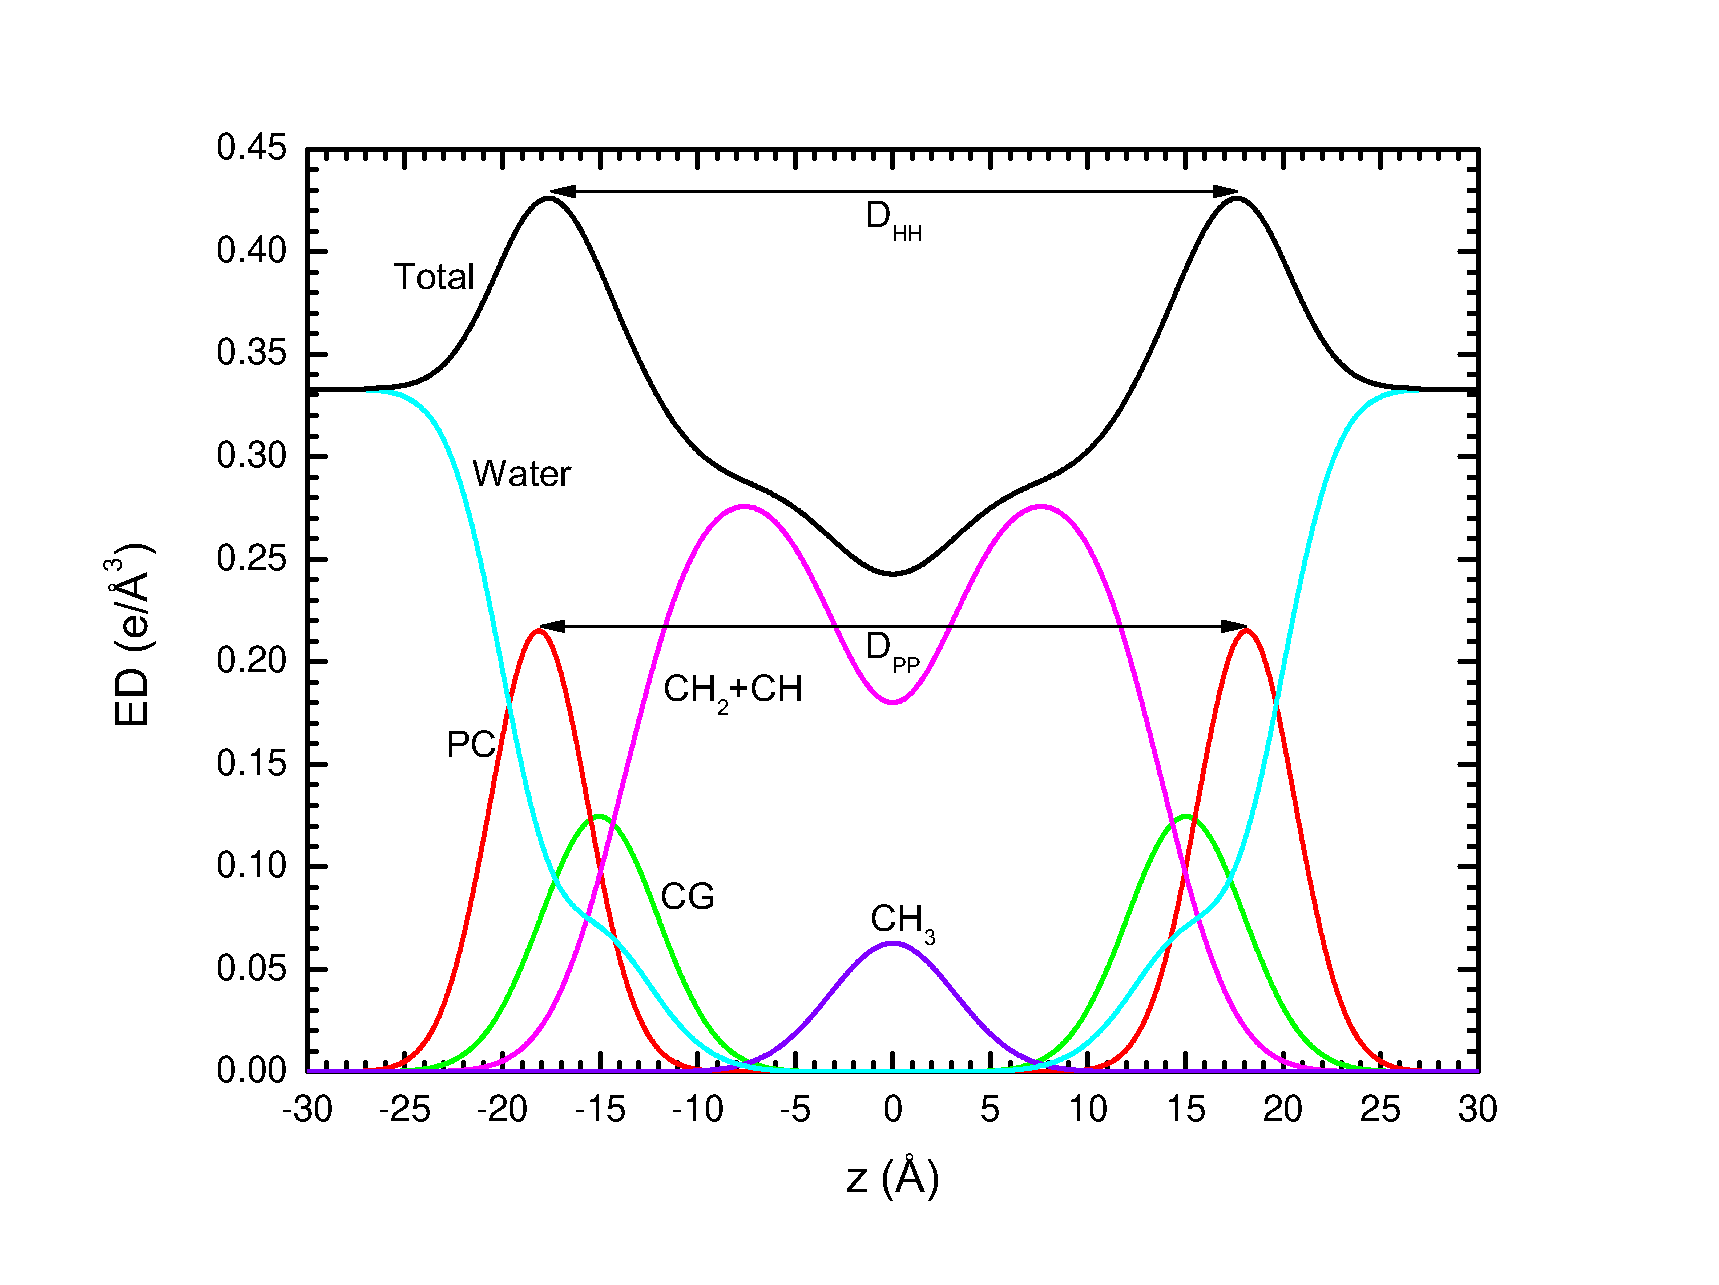
\includegraphics[scale=0.3]{./figures/SDP_Results/DOPC_EDP1.pdf}
  \caption{DOPC electron density (ED) profile}
  \label{fig:DOPC_EDP1}
\end{figure}
%------------------------------------------------------------------------------
\begin{figure}[htbp]
  \centering
  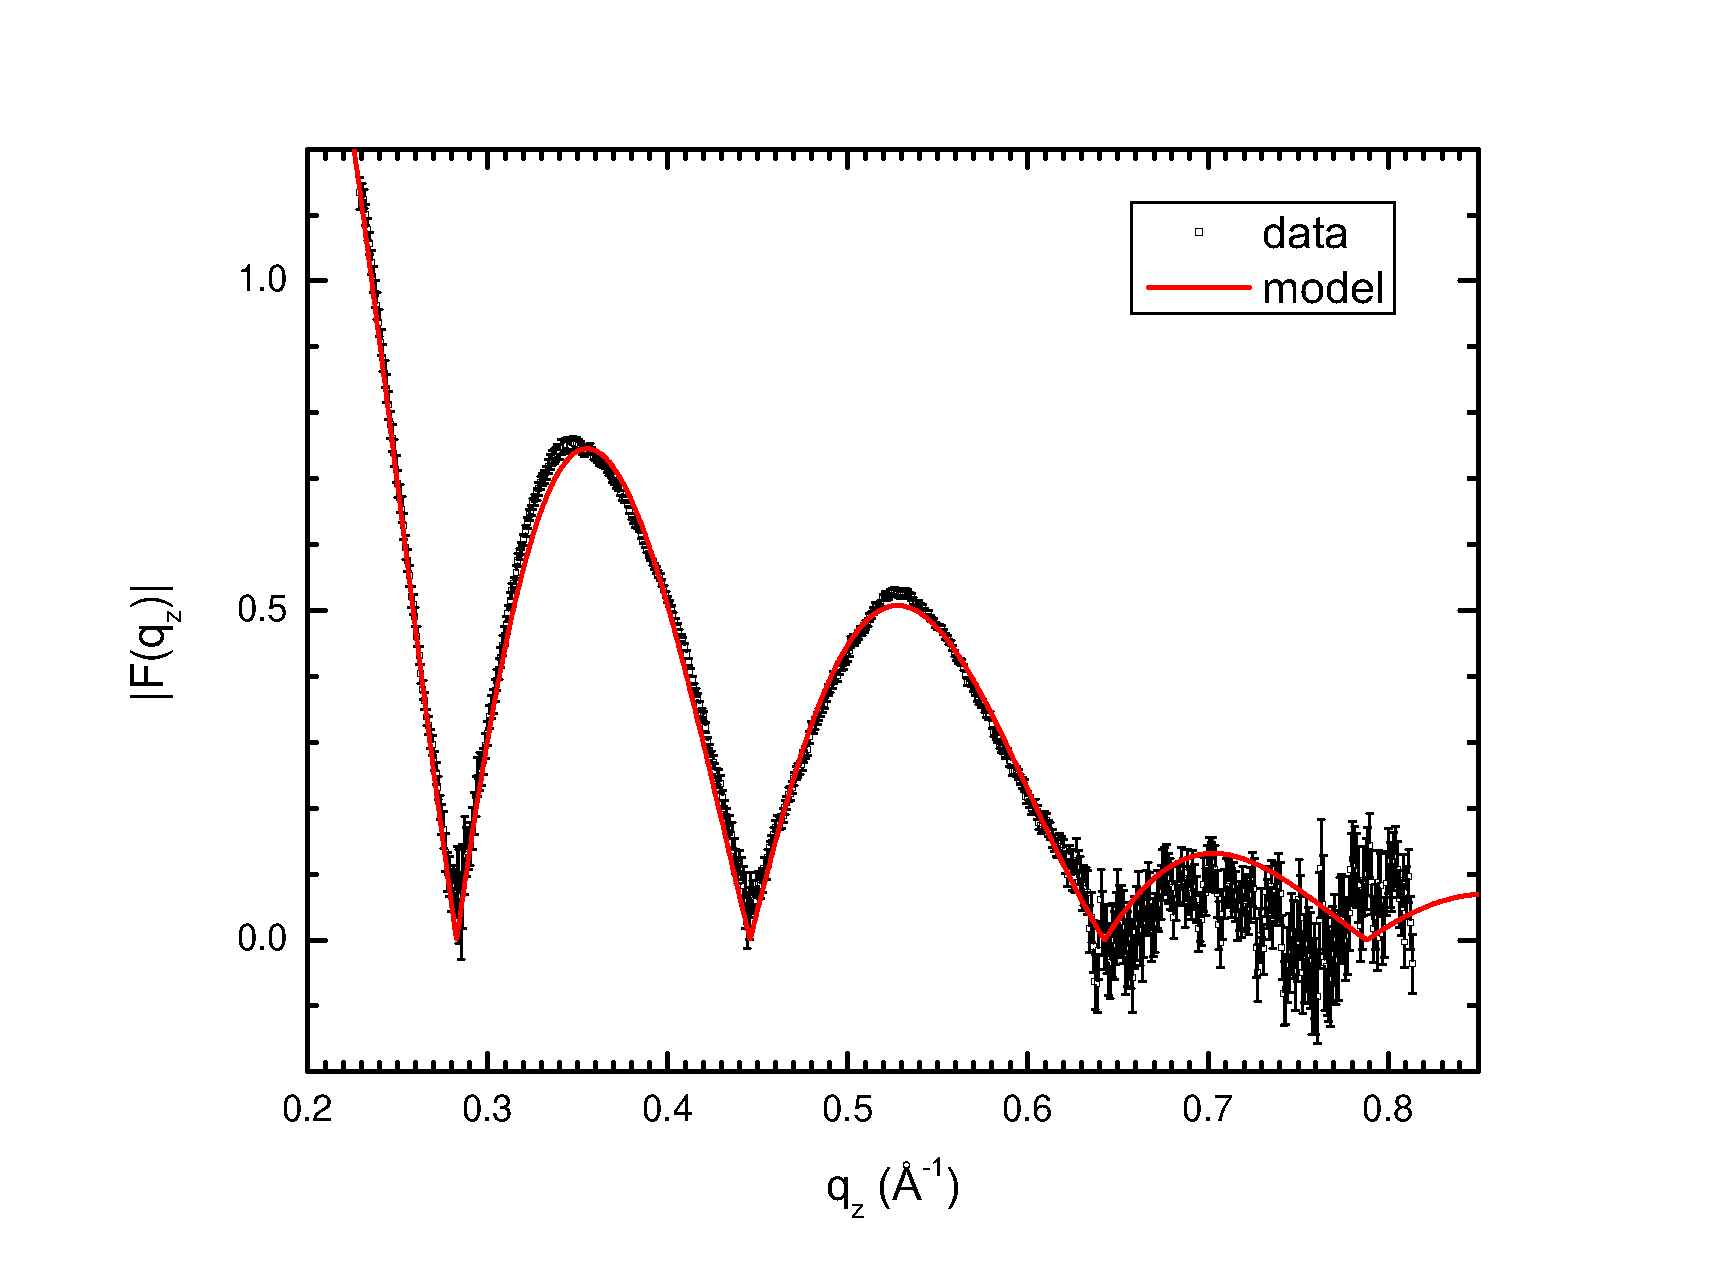
\includegraphics[scale=0.3]{./figures/SDP_Results/DOPC_XFF1.pdf}
  \caption{DOPC form factor}
  \label{fig:DOPC_XFF1}
\end{figure}
%------------------------------------------------------------------------------
(Table ? shows the best fit parameters for DOPC bilayers. Explain the 
constraints on the distance between the headgroup components.)

For fitting the form factors for systems with Tat, we fixed the width of Tat 
Gaussian because we found that the best fits of this width was always 
unphysically too small. We fitted with three different values of widths,
2.5, 3.0, and 3.5, to study the range of variation due to the Tat width. 
The choice was made based on MD simulation results. (Check this again)
Figure~\ref{fig:DOPC_Tat_62to1_3.0_XFF1} shows the best fit to the 
form factor for DOPC:Tat (62:1). 
%------------------------------------------------------------------------------
\begin{figure}[htbp]
  \centering
  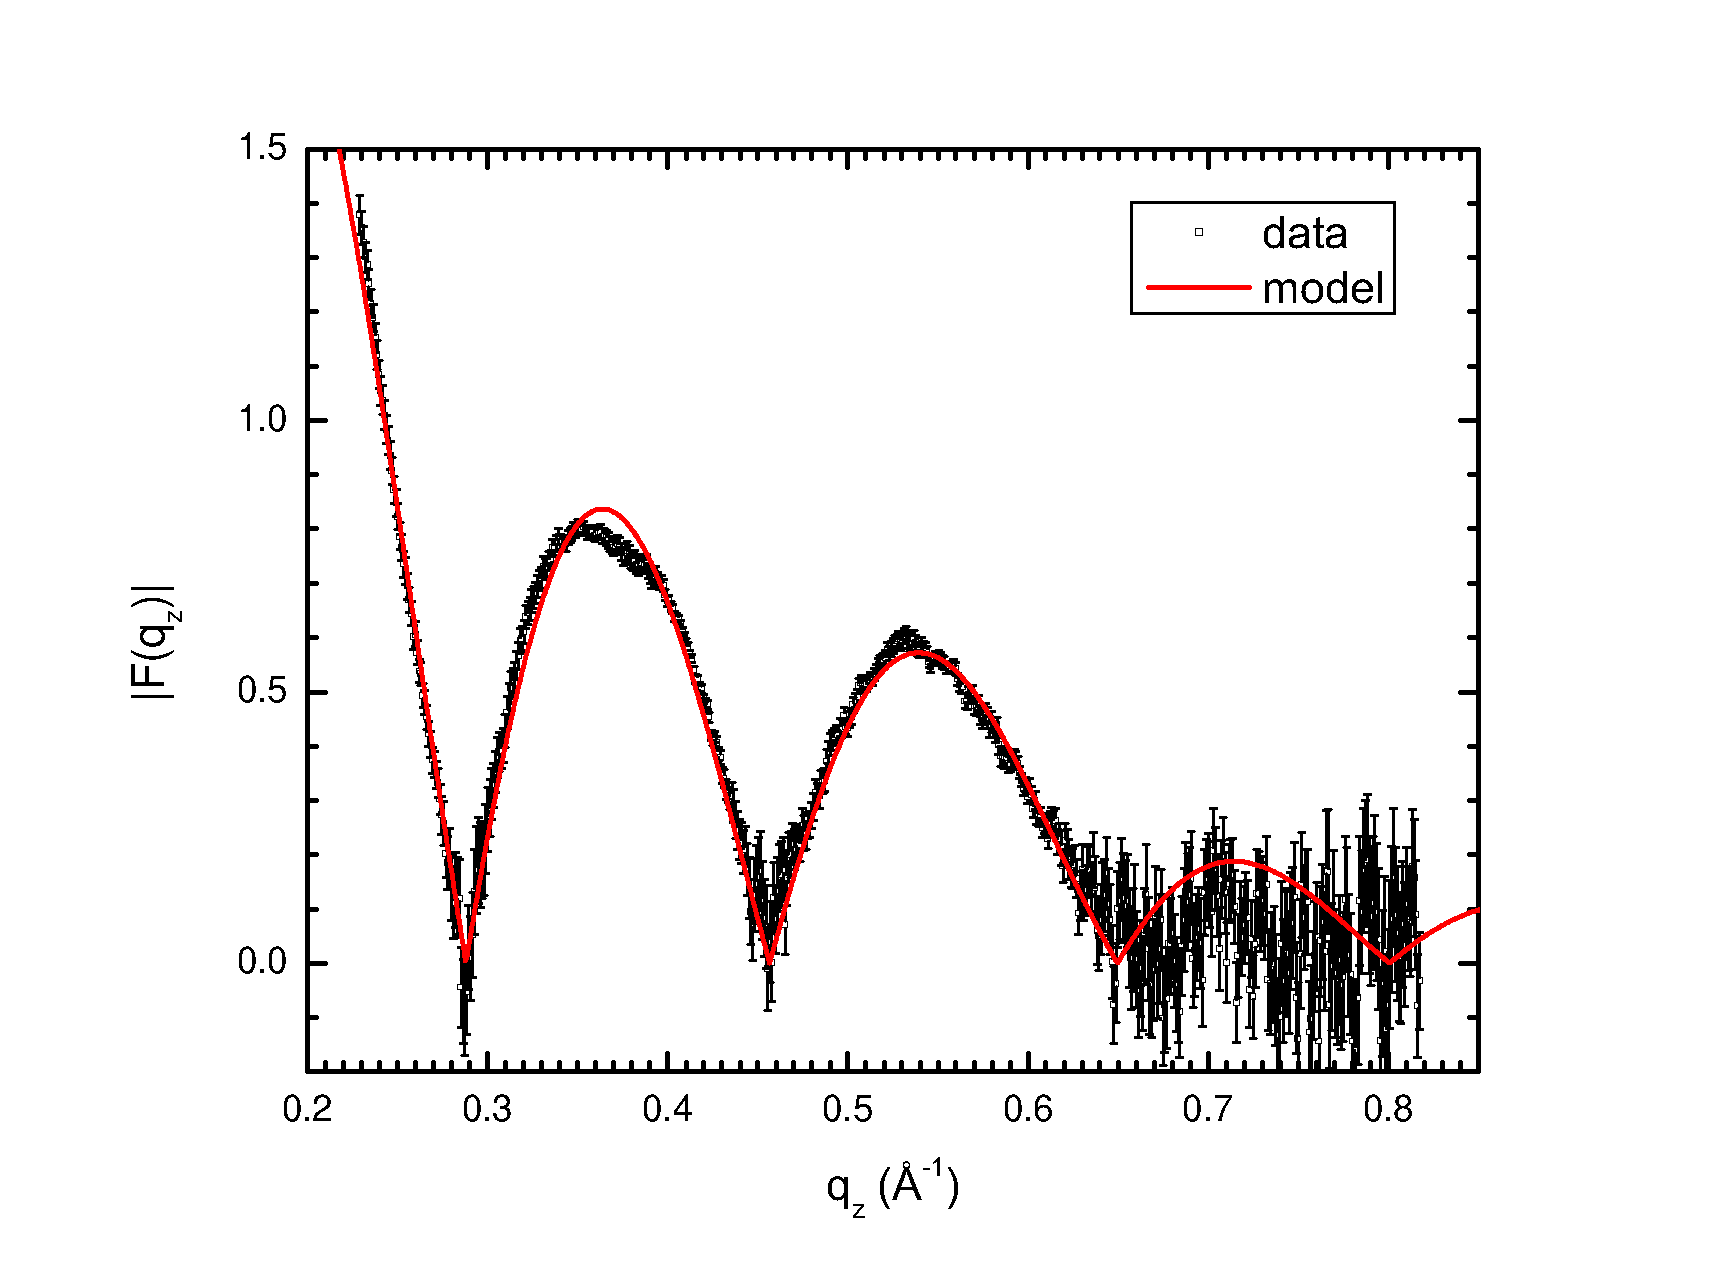
\includegraphics[scale=0.3]{./figures/SDP_Results/DOPC_Tat_62to1_3_XFF1.pdf}
  \caption{DOPC:Tat (62:1) form factor}
  \label{fig:DOPC_Tat_62to1_3.0_XFF1}
\end{figure}
%------------------------------------------------------------------------------
\begin{figure}[htbp]
  \centering
  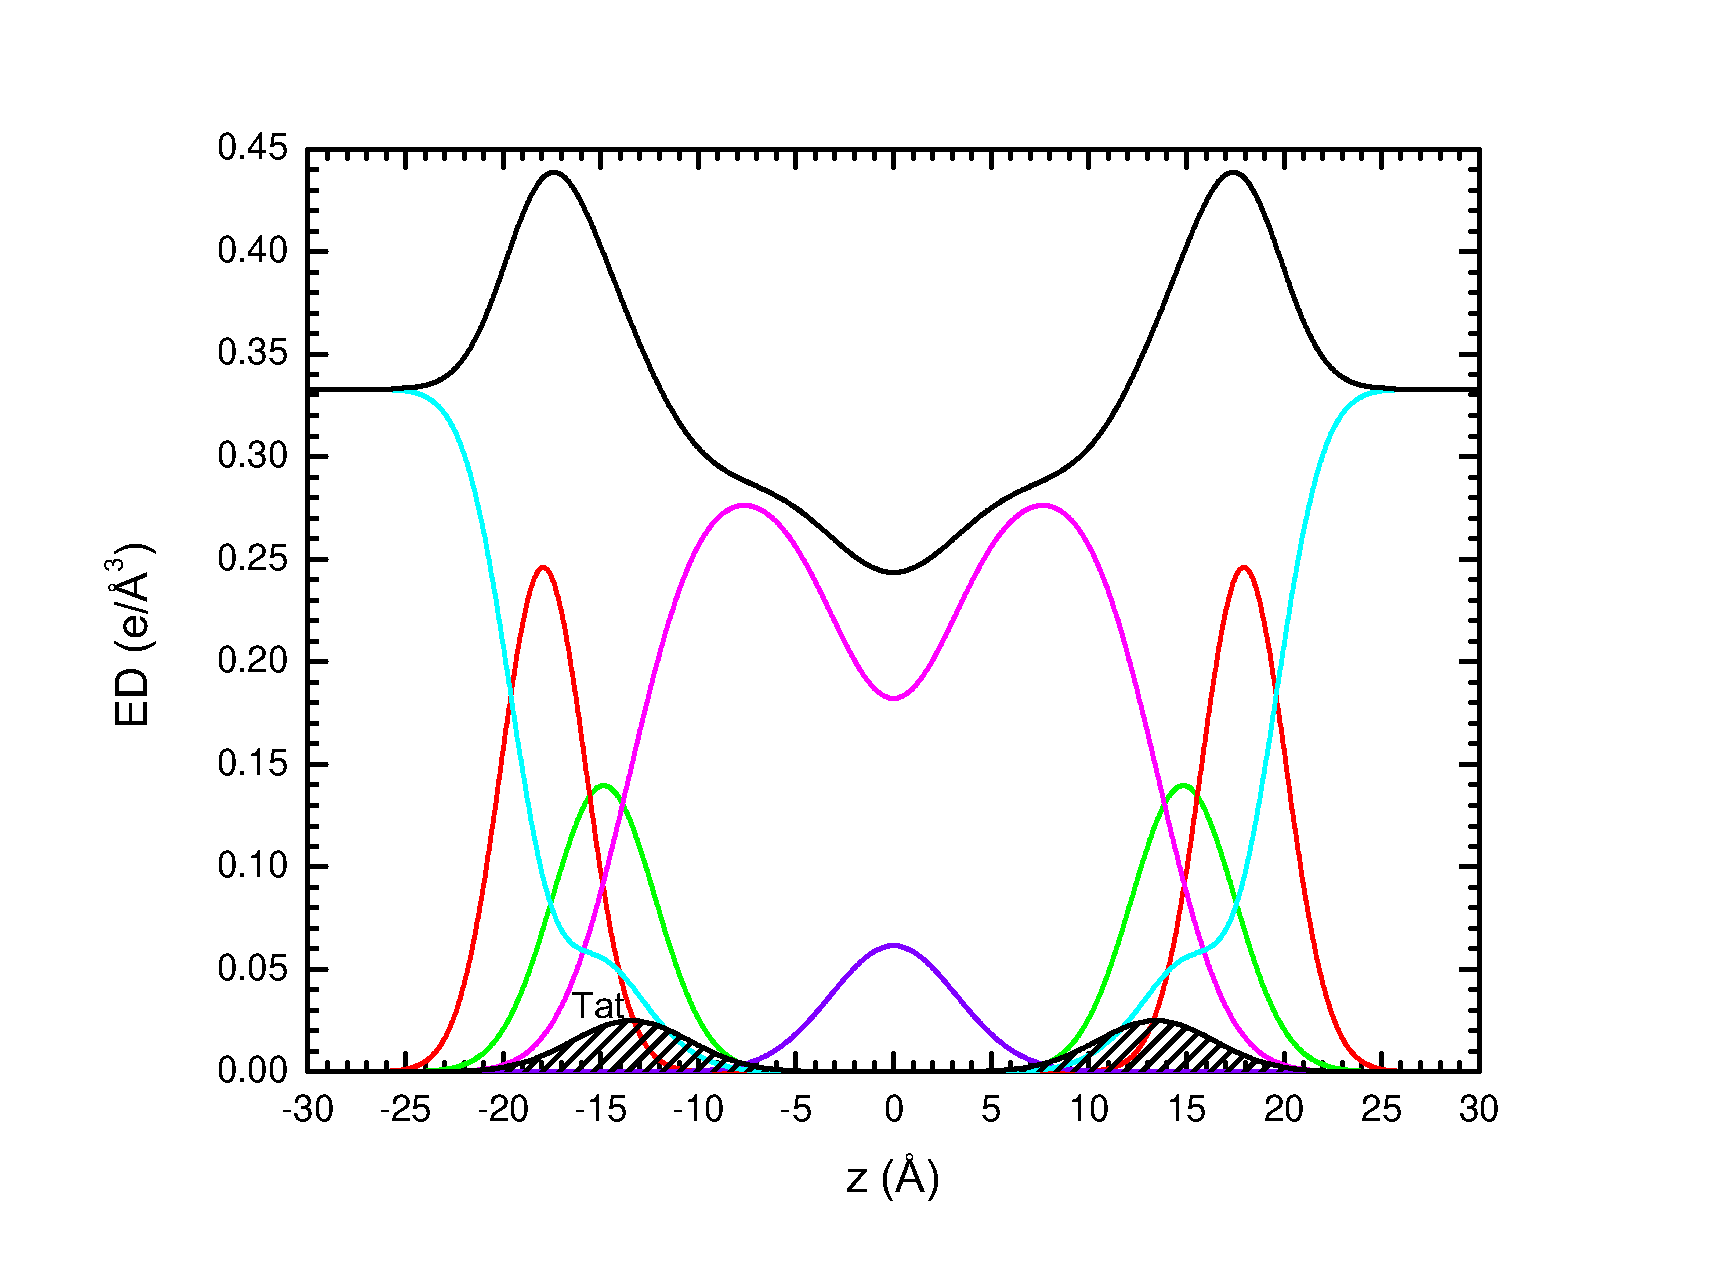
\includegraphics[scale=0.3]{./figures/SDP_Results/DOPC_Tat_62to1_3_EDP1.pdf}
  \caption{DOPC:Tat (62:1) ED profile. Colors are the same as in 
  Fig.~\ref{fig:DOPC_EDP1}}
  \label{fig:DOPC_Tat_62to1_3.0_EDP1}
\end{figure}
%------------------------------------------------------------------------------
(Show all the results in a composite figure. Show results for DOPC:DOPE bilayers.)

Figure~\ref{fig:DOPC_Tat_62to1_X2} shows $\chi^2$ as a function of fixed Tat position, 
$\zTat$. Generally, two minima were found. For DOPC bilayers, $\zTat$ in the 
headgroup region yielded the best fit. (Show plots for DOPC bilayers)
%------------------------------------------------------------------------------
\begin{figure}[htbp]
  \centering
  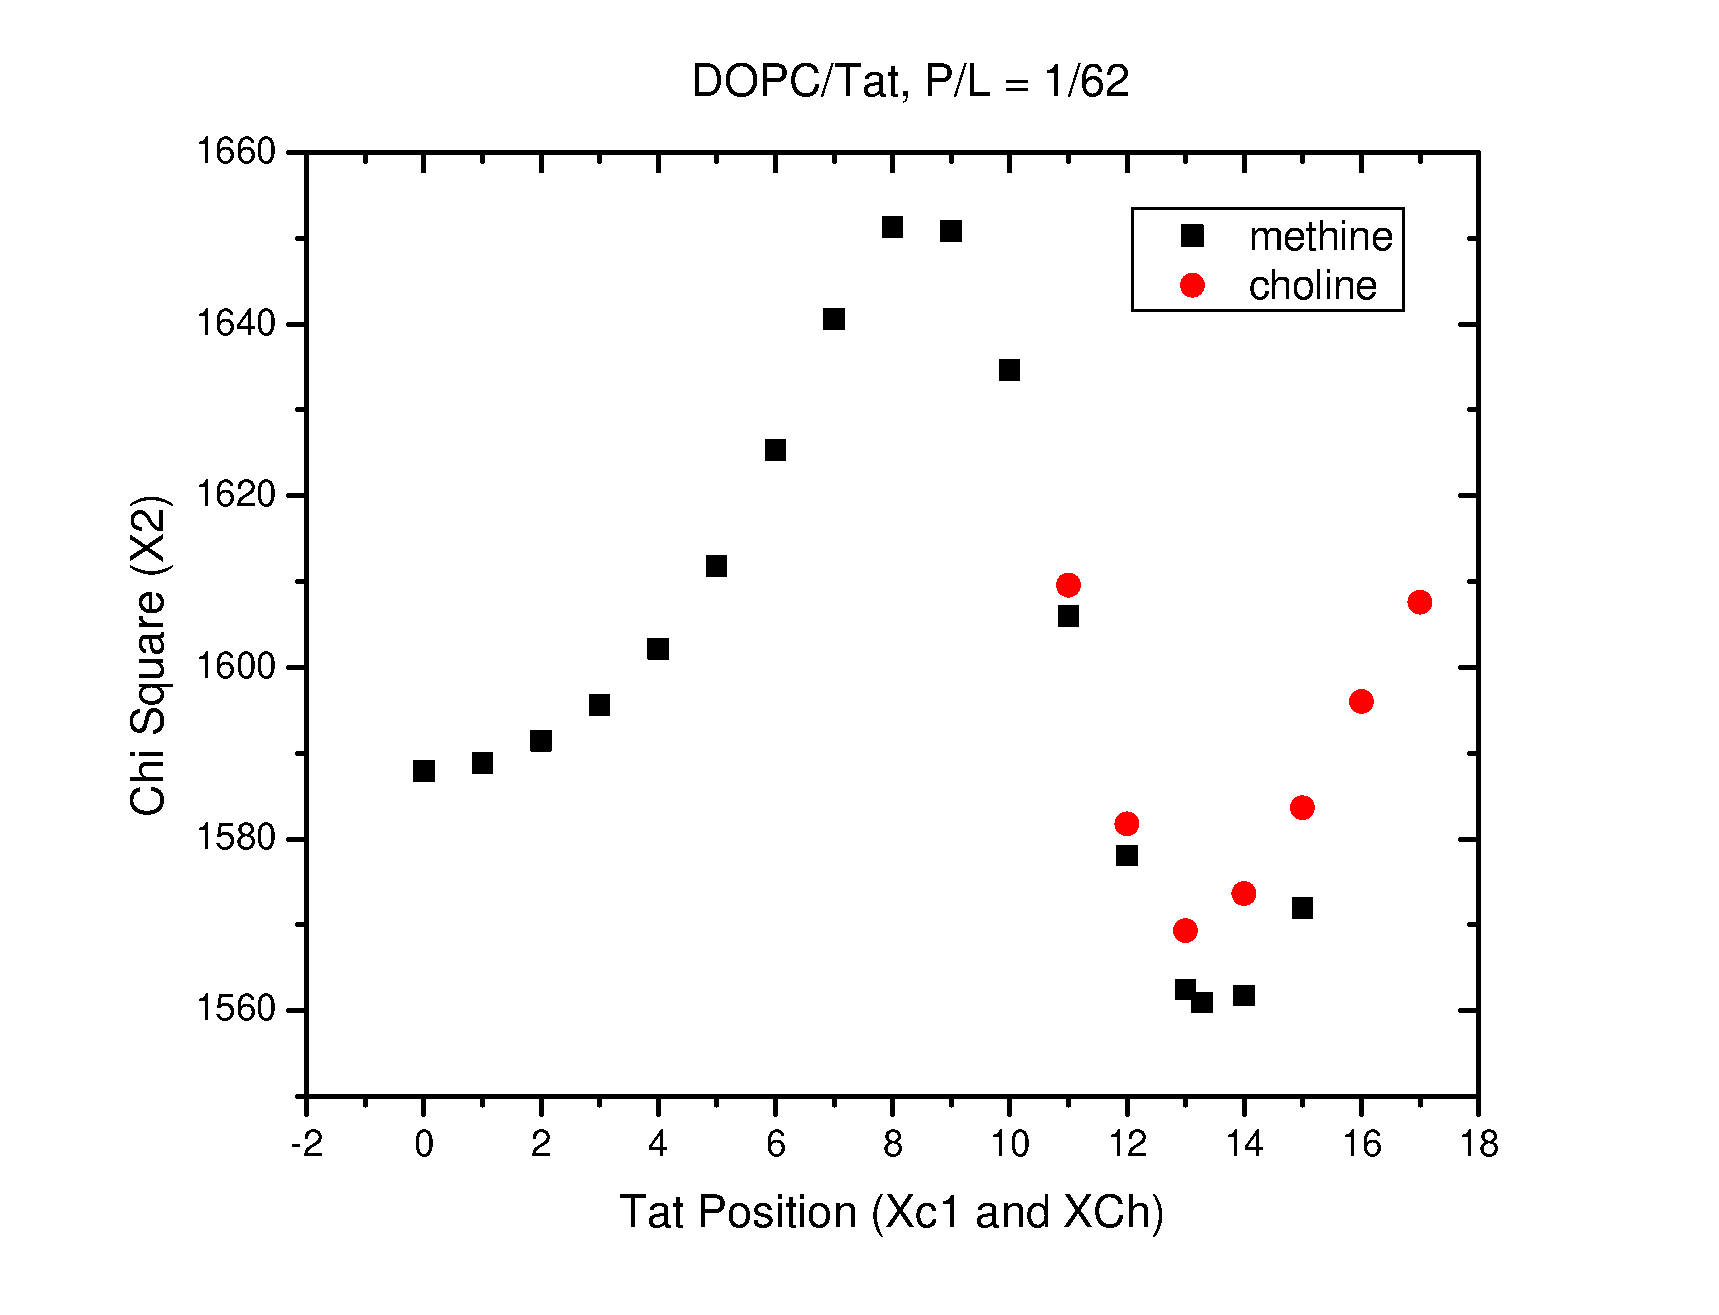
\includegraphics[scale=0.3]{./figures/SDP_Results/DOPC_Tat_62to1_X2.pdf}
  \caption{$\chi^2$ as a function of $\zTat$ for DOPC:Tat (62:1).}
  \label{fig:DOPC_Tat_62to1_X2}
\end{figure}
%------------------------------------------------------------------------------
\begin{figure}[htbp]
  \centering
  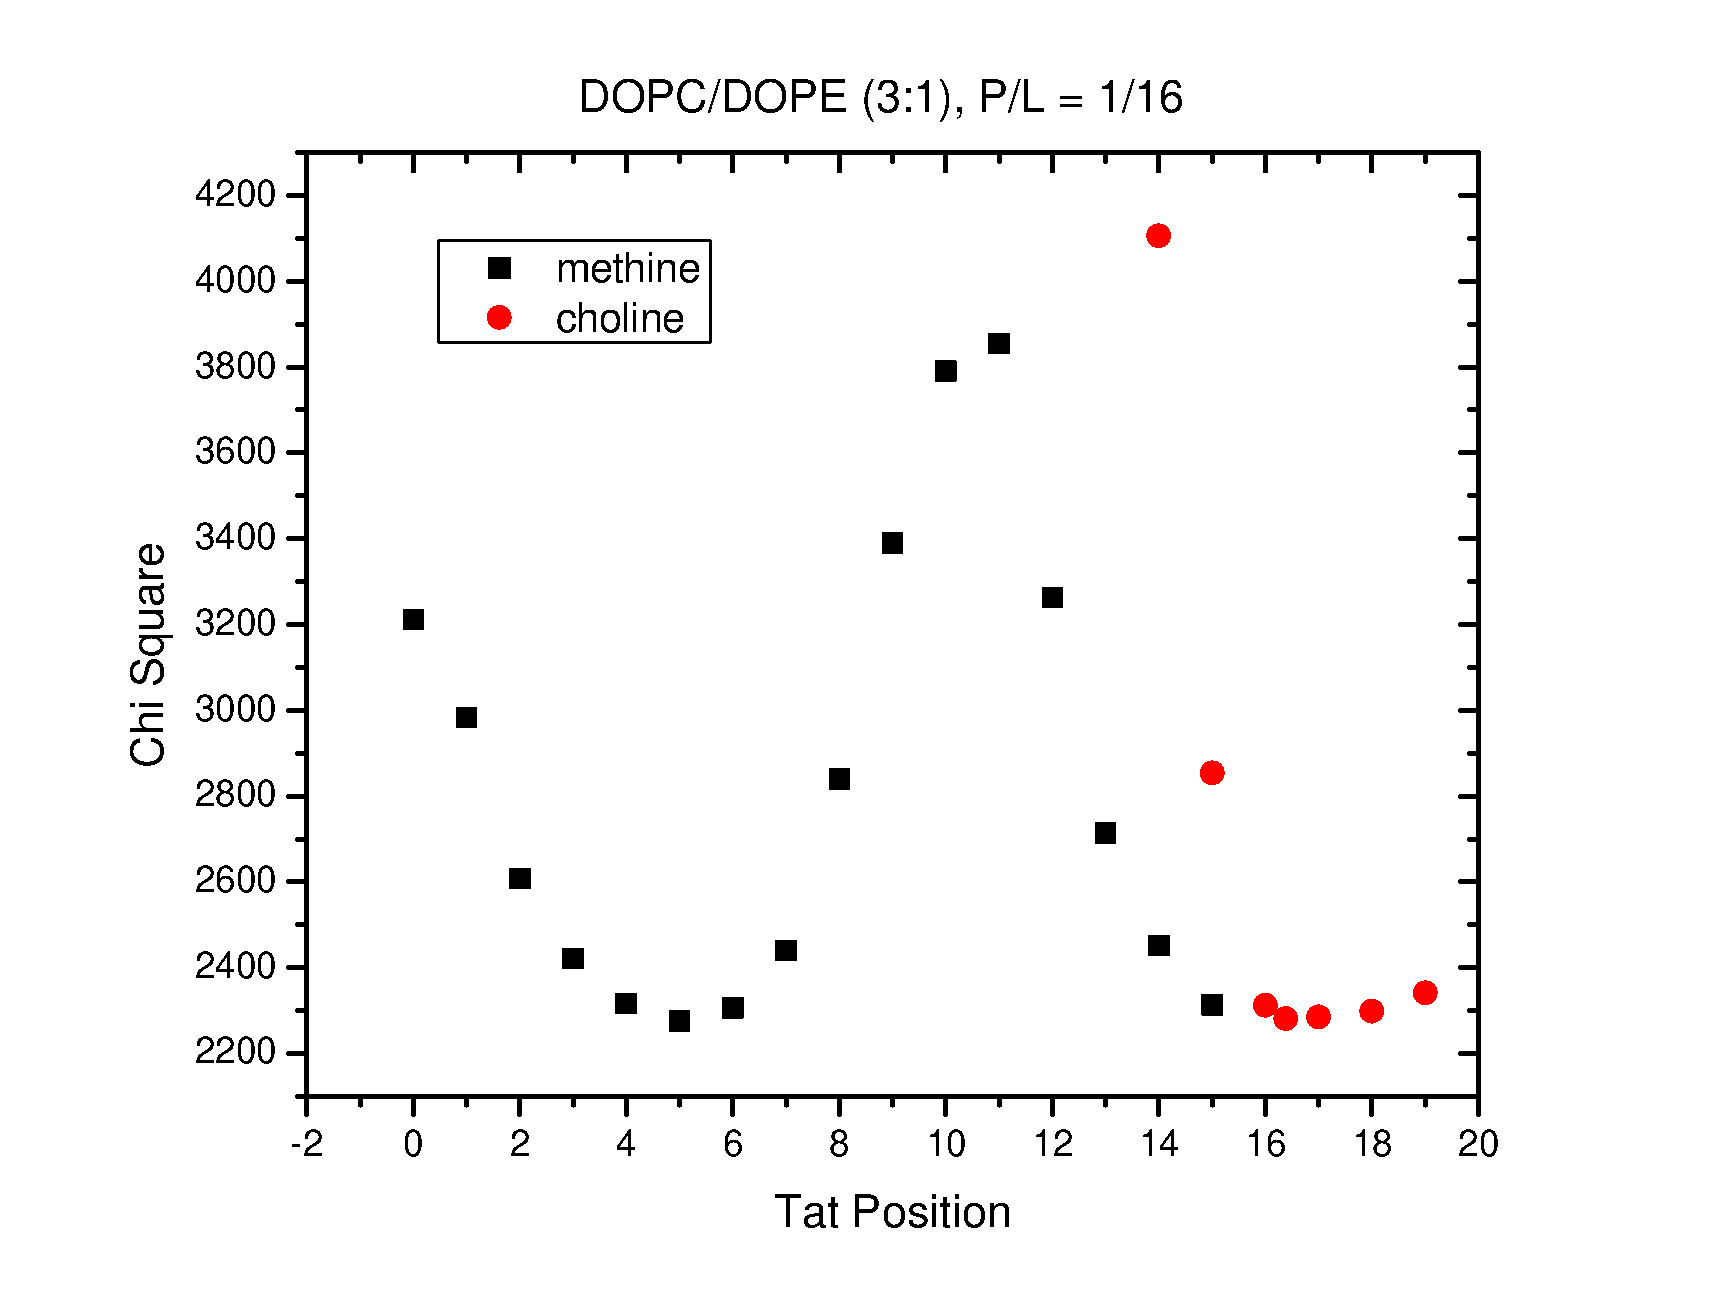
\includegraphics[scale=0.3]{./figures/SDP_Results/DOPCDOPE3to1_Tat_16to1_X2.pdf}
  \caption{$\chi^2$ as a function of $\zTat$ for DOPC:DOPE (3:1) with 
  $x_\textrm{Tat}=1/17$, where $x_\textrm{Tat}=Tat/(Tat+Lipid)$.}
  \label{fig:DOPCDOPE3to1_Tat_16to1_X2}
\end{figure}
%------------------------------------------------------------------------------
However, as Fig.~\ref{fig:DOPCDOPE3to1_Tat_16to1_X2} shows, the fits are are 
equally good with Tat inside and outside the chain region for DOPC:DOPE bilayers.
(Show a bunch more plots for DOPC:DOPE membranes) 
While modeling suggested
that Tat could be in the tail region, this position seems energetically 
unfavorable as Tat is a hydrophilic molecule. With a help of MD simulations,
we were able to discard the interior position as an artifact of our 
modeling. The simulation results are discussed later.

%%%%%%%%%%%%%%%%%%%%%%%%%%%%%%%%%%%%%%%%%%%%%%%%%%%%%%%%%%%%%%%%%%%%%%%%%%%%%%%
\newpage
\section{Volume Measurements}
(Maybe do this in appendix?)

%%%%%%%%%%%%%%%%%%%%%%%%%%%%%%%%%%%%%%%%%%%%%%%%%%%%%%%%%%%%%%%%%%%%%%%%%%%%%%%
\newpage
\section{MD simulation}
Three systems with different petpide concentrations (DOPC:Tat = 128:0, 128:2, and 128.4)
were studied with Gromacs 4.6.1 package \cite{ref:Hess08}. DOPCs were modeled by Slipid 
force field \cite{ref:Jambeck12_JPCB,ref:Jambeck12_JCTC} and HIV-Tats
were modeled by Amber99SB \cite{ref:Hornak06}. The systems were simulated at 
310 K with a constant
area in the x-y plane. The z direction was coupled to 1 atm with constant pressure. The
center of mass (COM) distance between each peptide and the bilayer was constrained by an
umbrella potential with a force constant of 3000 kJ/mol/nm$^2$. Each system was explored
18 independent simulations as a combination of 3 different constant area and 6 different
peptide insertion depths (except the pure DOPC system).

\begin{equation}
  z_{\mathrm{cm}} = \frac{\sum\limits_{i=1}^N m_iz_i}{\sum\limits_{i=1}^N m_i}
\end{equation}
The center of mass constraint was applied through an external force field,
which derives from an added pontential energy of the system. The pontential 
is like a spring, where it depends on the deviation of the distance 
between the center of mass of Tat and DOPC from a prefered value, $z_0$,
\begin{equation}
  U(z_1^{\Tat},\ldots,z_1^{\DOPC},\ldots) = 
  -\frac{1}{2} k 
  \pars{z_{\cm}^{\Tat} - z_{\cm}^{\DOPC} - z_0}^2
\end{equation}
Then, $-\partial U/\partial z_i$ is equal to the external force acting 
on atom, $i$. Before applying this constraint, Tats were attached to 
the bilayer from the water region. During the first 20 ns for 
pre-equilibration, Tats were allowed to change their configuration,
which resulted in different configurations for each Tat when attached
to the bilayer. It is possible that the Tats configuration inside the
bilayer at the end of simulations was affected by this initial 
configuration of Tats. Instead of preparing many simulations with
different initial Tat configurations, we avaraged over all Tats
present in the system. We also performed many simulations with
different $A_L$ and $z_{\Tat}$ to investigate how robust some of the 
Tat structural features are. Many simulation results are shown in
the appendix of this thesis. 


%%%%%%%%%%%%%%%%%%%%%%%%%%%%%%%%%%%%%%%%%%%%%%%%%%%%%%%%%%%%%%%%%%%%%%%%%%%%%%%
\subsection{Local Thinning of Membranes}
The SIMtoEXP program only gives the average quantities for each leaflet. 
While our x-ray data are sensitive to the avarage bilayer electron density,
local information of Tat-DOPC interactions can be obtained from MD simulations.
In this section, we discuss a method to extract a local membrane thickness.

The presence of Tat may result in compression of lipid bilayer along z-direction. 
If so, the phosphorus-phosphorus distance of the bilayer near Tat (denoted by DPP'
in the figure below) may be different from that away from Tat (DPP).  For 
small Tat concentration, DPP would be the same as that of pure DOPC if the 
distance from all Tats is large enough.  Of course, for our concentrations, 
the thinning effect may extend throughout the bilayer because the lateral
effect of Tat might have a larger lateral decay length than the distance 
between Tats.  Whether that is the case or not, one would expect that the 
thickness near the Tats is smaller than the average thickness.

\begin{figure}[htbp]
  \centering
  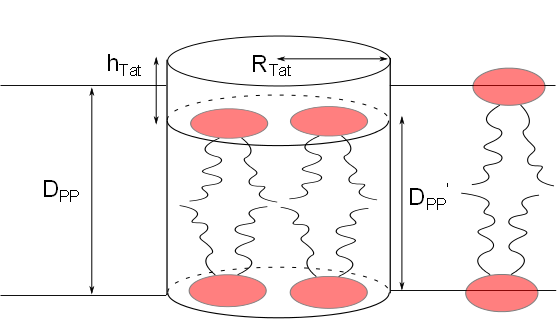
\includegraphics[scale=0.5]{./figures/cylinder_model}
  \caption{test}
  \label{fig:cylinder_model}
\end{figure}
So, we want to measure DPP'.  First, let us define what we mean by lipids 
close to Tat.  As in Fig.~\ref{fig:cylinder_model}, we imagine a cylinder around Tat and 
pick up all the phosphorus atoms within it.  Approximating Tat as a cylinder 
with its height given by the FWHM of its electron density distribution, its 
radius $R_\mathrm{Tat}$ = 9~\AA\ comes from the volume of Tat = 1876~\AA$^3$ and 
$\hTat$ = 7.6~\AA\
measured from one of the simulations. Let us define the lateral center of the 
cylinder in some way - a crude approximation would put it at the arginine in 
the middle of the amino acid sequence. Then let us define DPP' using only 
those lipids whose phosphorus atoms lie within these 9\AA\ cylinders around the 
tats. Then $D_\mathrm{PP} = \zphos^+ - \zphos^-$ where $\zphos^+$ and $\zphos^-$ 
are the 
average $Z$ of the n1 (n2) lipids in the upper and lower monolayer, respectively.  
To be more precise, assume that the arginine in the middle of the amino acid 
sequence is at the center of the cylinder. For a refined method, we could find 
the center of mass of each Tat and use them as the lateral center of cylinders 
(instead of a particular carbon atom in an arginine). 

The algorithm for doing this is straightforward.  For each time frame 
(snapshot), the positions ($X_i$ ,$Y_i$, $Z_i$) of each Tat, $i$, are listed.   
We choose phosphorus atoms whose ($X$, $Y$) lateral position lies within 
9~\AA\ of any one of the Tat's lateral position. Then, $Z$ position
of the chosen phosphorus atoms are placed in a 
list. Then, $\zphos$ are calculated from the list. 
The number of selected phosphorus atoms in each monolayer was also 
recorded. This value gives local lateral depletion if the Tat cylinders 
are assumed not to overlap. After averaging over many snapshots, 
there will hopefully be decent statistics 
for local thinning and local difference between Tat and phosphorus Z positions, 
and maybe local lateral depletion if overlaps are taken into account.  

\subsection{Linear Model}
As described in the previous section, a Tat is modeled as a cylinder with 
its radius equal to $R_1$, height $\hTat$,
and volume $\VTat$ such that $R_1=\sqrt{\VTat/(\pi \hTat)}$. 
Let $h(r)$ represent the phosphorus height profile
of a leaflet. The two leaflets are assumed to be decoupled.
In the linear model, lipids are seprated into three regions: 
suppressed, boundary, and unperturbed (see Fig. for the definitions
of various quantities). 
%------------------------------------------------------------------------------
\begin{figure}[htbp]
  \centering
  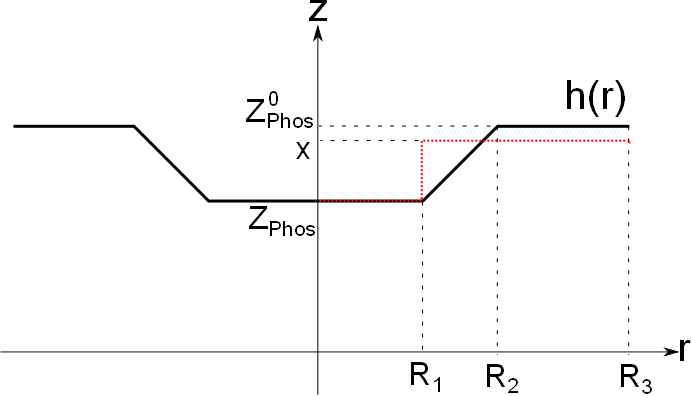
\includegraphics[scale=0.5]{./figures/linear_model.png}
  \caption{test}
  \label{fig:linear_model}
\end{figure}
%------------------------------------------------------------------------------
In the suppressed region,
lipids are uniformly compressed by Tat toward the center of the bilayer; 
$h(r)$ is a constant, $\zphos$. In the boundary region, $h(r)$ is assumed to 
linearly increase with the distance $r$ from the center of the Tat. In
the unperturbed region, lipids do not interact with Tat, behaving
identially to DOPC, so the phosphorus position is the same as that of 
DOPC. A continuous $h(r)$ that 
satisfies the above criteria is
\begin{equation}
  h(r) = \left\{ 
  \begin{array}{lcr}
    \zphos   & \text{if} & 0   \leq r < R_1 \\
    mr+b     & \text{if} & R_1 \leq r < R_2 \\
    \zphos^0 & \text{if} & R_2 \leq r < R_3 
  \end{array}\right.  
\end{equation}     
with $m=(\zphos-\zphos^0)/(R_1-R_2)$ and $b=(\zphos^0R_1-\zphos R_2)/(R_1-R_2)$. 
Assuming that the simulation box is a cylinder, we have 
$R_3=\sqrt{N\AL/\pi}$. $\zphos$ can be measured directly from simulation trajectories.
$\zphos^0$ is a half of the average phosphorus-phosphorus distance in a DOPC simulation,
which can be easily obtained from the SIMtoEXP program. The average height profile over
the monolayer, $\langle h(r) \rangle$, can be also obtained from the program in the same manner. 
The only unknown is $R_2$, which is the relaxation length of DOPC-Tat interaction.

Let us calculate $\langle h(r) \rangle$. In the cylindrical coodinates, 
\begin{equation}
  \langle h(r) \rangle 
  = \frac{1}{\pi R_3^2} \int_0^{2\pi}d\phi \int_0^{R_3}\dr rh(r)
\end{equation}
The $\phi$ integration is trivial. The $r$ integration is
\begin{align}
  & \int_0^{R_3}\dr rh(r) \nonumber\\
  &= \int_0^{R_1}\dr \zphos r + \int_{R_1}^{R_2}\dr (mr+b)r + \int_{R_2}^{R_3}\dr \zphos^0r \nonumber\\
  &= \frac{1}{2}\left[\zphos R_1^2+\zphos^0(R_3^2-R_2^2)\right] + 
     \frac{1}{3}m\left(R_2^3-R_1^3\right) + 
     \frac{1}{2}b\left(R_2^2-R_1^2\right) \nonumber\\        
  &= \frac{1}{2}\left[\zphos R_1^2+\zphos^0(R_3^2-R_2^2)\right] +
     \frac{1}{3}\left(\zphos^0-\zphos\right)\left(R_2^2+R_1R_2+R_1^2\right) \nonumber\\
  &  + \frac{1}{2}\left(\zphos R_2-\zphos^0 R_1\right)\left(R_1+R_2\right) \label{eq:r_integ}
\end{align}
Using Eq.~(\ref{eq:r_integ}), we get 
\begin{equation}
  \langle h(r) \rangle 
  = \frac{\left(\zphos-\zphos^0\right)\left(R_1^2+R_1R_2+R_2^2\right)+3\zphos^0R_3^2}{3R_3^2}
  \label{eq:quadR2}
\end{equation}
Eq.~\ref{eq:quadR2} is a quadratic equation in terms of $R_2$. 
Solving for $R_2$ gives
\begin{equation}
  R_2 = \frac{-R_1+\sqrt{R_1^2+4C}}{2} 
\end{equation}
with
\begin{equation}
  C = \frac{3R_3^2\left(\zphos^0-\langle h(r)\rangle\right)}{\zphos^0-\zphos} - R_1^2
\end{equation}
The model quantities calculated from the MD simulations are shown in Table.

%%%%%%%%%%%%%%%%%%%%%%%%%%%%%%%%%%%%%%%%%%%%%%%%%%%%%%%%%%%%%%%%%%%%%%%%%%%%%%%
\newpage
\section{Discussion}
We also estimated the structure by fitting the experimental form factors to a 
model using the SDP method with the component groups identified in Fig. (what  
The positions of 
these groups were free parameters and the agreement with the experimental form 
factors was excellent (see Fig. S.M. 5).  Absolute total electron density 
profiles and the Tat profiles are shown for many samples in Fig. 6 (A-C).  
It must be emphasized, however, that, while the total EDP is well determined by 
this fitting procedure.  Indeed, there are local minima in the fitting landscape, 
including one with Tat closer to the center of the bilayer as shown in Fig. 
S.M. 5.  The simulations help to discard that result. For the results shown in 
Fig. 6, a consistent trend is that Tat moves away from the bilayer center as 
concentration increases. 

Figure shows that $A_L$ as defined by $(V_L-V_{HL})/D_c$ decreases as the 
amount of DOPE increases for systems without Tat. This is consistent with the
previous studies (or predictions?) and attributed to the small size of PE
head group. Because DOPE has smaller head group than DOPC, lipids in DOPC/DOPE
bilayers pack more compactly than DOPC bilayers do, leading to a smaller $A_L$.
Consequently, bilayers composed of DOPC and DOPE tend to have a higher order 
parameter than DOPC alone. (NO THEY DON'T. WHAT'S GOING ON HERE?). Similarly,
the thickness of bilayers is larger at higher PE content. 

Figure shows that Tat is located further out from the bilayer center with 
higher content of PE lipids. This is also consistent with MD simulation PMF,
which showed that arginine insertion cost more energy for PE membrane than
PC membrane, the result of which was attributed to more possible hydrogen 
bonding between PE group and arginines.



More structural detail from the modeling and from the simulations is shown in 
Fig. 7. The bilayer thickness can be described as DHH, which is the 
distance between the maxima in the electron density profile, or as DPP, which 
is the distance between the phosphocholines on the opposing monolayers. Figs. 
7A and 7B show that both these quantities decrease with increasing Tat mole 
fraction (P/(L+P)), showing that Tat thins membranes, increasingly so as its 
concentration is increased, even though both simulation and modeling suggest 
that Tat moves further from the membrane center with increasing concentration 
as shown in Fig. 7D.  Fig. 7C shows that the area per lipid AL usually increases 
with increasing mole fraction of Tat, as would be expected from consideration of 
conservation of lipid volume. Interestingly, the bilayer thickness did not 
increase for DOPC/DOPE (3:1) bilayers with x less than 0.03.  

Figure 8 shows that the Sxray orientational order parameters generally 
decreases with increasing concentration of Tat for most of the membrane mimics 
studied.  These decreases in membrane chain order are compatible with the 
increase in softening of membranes by Tat observed by a decrease in the bending
energy, KC, in Fig. 2.

\section{Conclusion}

\bibliography{Tat}
\bibliographystyle{unsrt}
%\bibliographystyle{plain}
%\bibliographystyle{abbrv}
%\bibliographystyle{alpha}
%\printbibliography

\end{document}
